\section{Proposed System Model}
\label{c:system_model}

\begin{figure}[!t]
\centering
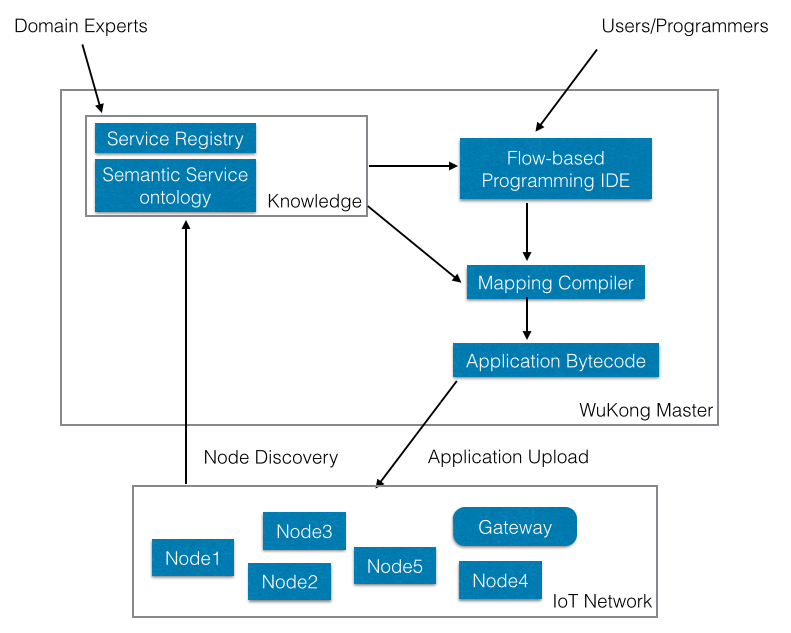
\includegraphics[width=1.0\columnwidth]{five}
\caption{System structure of WuKong}
\label{fig_structure}
\end{figure}


In this section, we proposed WuKong, a service-oriented middleware in IoT. In our study, IoT systems are modeled as distributed system with sensor/actuator/virtual computing components devices that are deployed on different locations in a target environment and connected via RF communication channels. There is a policymaker, called WuKong master, standing on top of the underlying distributed system as figure \ref{fig_structure} shows. WuKong master takes the responsibility for coordinating and monitoring the underlying node devices. To address the challenges to separate virtual application with physical resources, we proposed three functional modules, knowledge base, FBP application IDE, mapping compiler. We elaborate each of them in turns. 

% Master下的knowledge Base
\subsection{Knowledge Base}

The most important part for WuKong master is the comprehensive understanding on top of its underlying distributed system. Master should be able to manage and configure the sensor nodes in a target environment. Based on this purpose, the knowledge of WuKong master consists of two parts, service definition, service registry.  

The definition of standard library of services should be part of the knowledge in WuKong master. The service with commonly-used primitive sensing or actuating or computing capability are defined as atomic service and called WuClass. Light sensor, light actuator, threshold can be examples for atomic services. Similiar to the class definition in object-oriented programming(OOP), we make definition of every atomic services for its functional properties and non-functional properties as figure \ref{fig:atomic} in XML format. Functional properties can be seen as the interface exposed by this service and are waiting to interact with other services. Non-functional properties can express the attributes and characteristics of the service. Non-functional properties will be updated as the IoT system runs. Example definition for atomic service is shown as follows: a temperature service has functional properties such as "readings" and 'refresh rate', non-functional properties such as 'power consumption', 'working range', 'sensitivity', 'precision', 'response time'. 

Compound service is a high-level service component that requires to be composed of several atomic services. In the definition for compound service, master should be aware of all possible substitutional solutions for it[圖2]. Foot step sensor can be seen as a high-level service component. There are several substitude FBP that can achieve the functionality of foot step sensor as defined in figure \ref{fig:compound}. such as and could be realized by either sound-level sensor or PIR sensor or camera sensor. 

% 一些會隨著the running of systems而改變的Property
A node device in IoT system can be equipped with more than one sensors/actuators. The master can generate virtual machine program according to device's capability and characteristics. After uploading it onto the sensor node, this node device can be called "available" to WuKong master because it can respond to master's query and configuration commands. A node device can host multiple services. At the first time to upload virtual machine program, non-functional properties for each residing service will be configureed. Some parameters such as network quality or device quality can vary as IoT system goes. After reasoning and learning process, WuKong master would adjust the parameters for each service on node device. 

\begin{figure}[!t]
\centering
	\begin{minipage}[t]{1.0\linewidth}
        \centering
        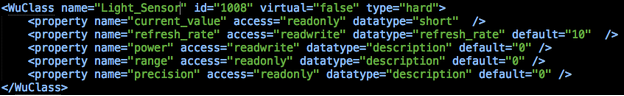
\includegraphics[width=1.0\columnwidth]{six}
        \caption{Example of atomic service definition as master knowledge base}\label{fig:atomic}
    \end{minipage}
    \\[0.2cm]
    \begin{minipage}[t]{1.0\linewidth}
        \centering
        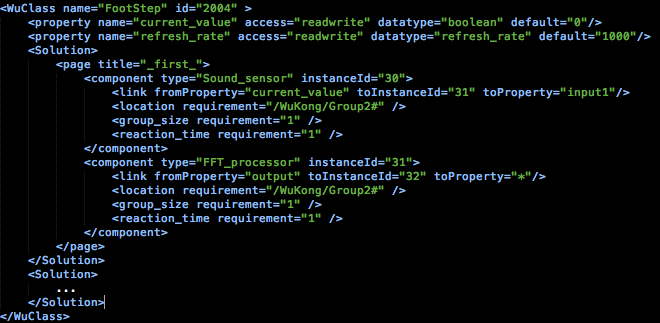
\includegraphics[width=1.0\columnwidth]{seven}
        \caption{Example of compound service definition as master knowledge base}\label{fig:compound}
    \end{minipage}
\end{figure}

\subsection{Flow based Programming IDE}

Most IoT applications are event-driven by nature. When there are some changes in sensors, events are created and passed from one part of IoT system to another. Therefore, the data and control flow should be the programming models for IoT applications as example FBP in figure \ref{fig_service_example}. Using FBP as programming model allow programmers focus on defining the abstract data flow in the application.  

The components that a programmer can use to compose the applications come from a pre-defined component library describe in master knowledge base. Componenets in FBP are defined by their abstract functionalities and interfaces. Each component can be regarded as a virtualized thing since it is possible to match with any physical device as long as the functionality is satisfied. Components can be connected using their exposed interfaces. 

%domain expert 

For each component, programmers can specify requirements so that WuKong master can take it into consideration when mapping. There are two kinds of user requirements described in our system. Point-based requirements are needed to be fulfilled definitely. For example, if the programmer want to get the temperature in living room, the component should be binded with temperature sensors or the device that can give temperature readings. Proximity-based requirements are not required to be fulfill completely but to express the level that the programmer cares for this property. The GUI for setting requirement is shown in figure \ref{requirement}. Programmer can express which properties should considered by selecting the check-box related the specific property. The position of slider is the priority of a property considered by programmer. The value of the slider ranges from 0 to 1. 0 represents that the property should be considered as lowest priority, while 1 stands for the property should be considered at top priority. 

For example, for a light sensor component, if programmer think this light sensor needs to be considered energy efficiency at top priority even if it sacrifices some of its performance, programmer will assign a weight for the power parameter to represent how much he/she cares for power of this component. After specifying point-based requirement and proximity-based requirement, we will do mapping for each service component for its best fit concrete service. 

\begin{figure}[!t]
\centering
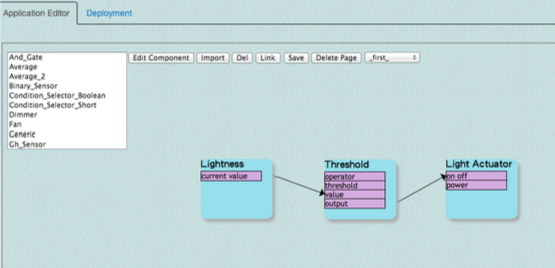
\includegraphics[width=1.0\columnwidth]{fbp}
\caption{The GUI for programming IDE}
\label{fig_sim}
\end{figure}


\begin{figure}[!t]
\centering
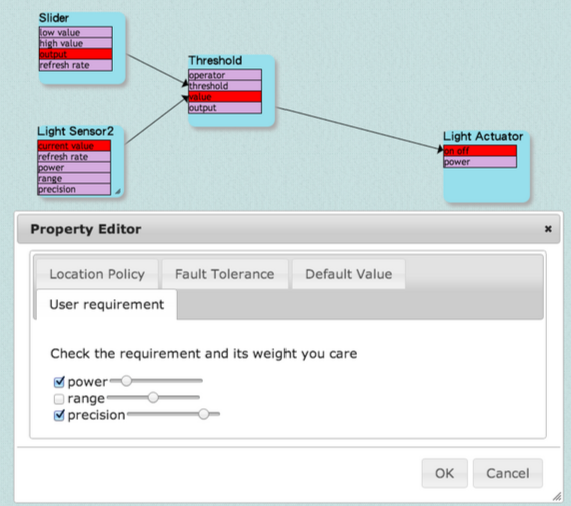
\includegraphics[width=1.0\columnwidth]{fbprequirement}
\caption{The GUI for choose weights}
\label{requirement}
\end{figure}



\subsection{Mapper}

After the programmer finish the application, FBP application IDE will export the application in XML file format. The mapper in WuKong master is to translate the application into hardware programs. After compressing the hardware programs to bytecodes, master then send bytecodes to corresponding node device and finish the application deployment. 

The flow of mapping should go by expansion, matchmaking for sensor/actuator component, matchmaking for computing component. In expansion phase, compound service should be expanded by a sub-FBP and connect to replace the original component. If there are multiple sub-FBP can replace the orignal component, then we should consider many FBPs and choose the best one in the end. 

\begin{figure}[!t]
\centering
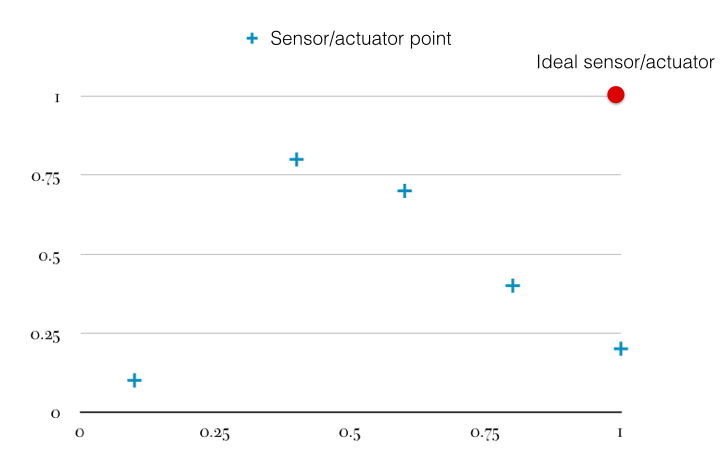
\includegraphics[width=1.0\columnwidth]{coordinate}
\caption{System structure of WuKong}
\label{fig:multidimensional}
\end{figure}

After expansion, we then perform one-to-one sensor/actuator matchmaking for each component. Matchmaking is a process that WuKong master decides the relationship between component and physical resource. Here we propose an user-oriented mapping scheme. Given the requirments provided by programmers, WuKong master will first filter all services from service repository by point-based requirement(e.g type, location). For the filtered result, we plot each candidate sensor/actuator on multi-dimensional space where each dimension is regarded as an attribute. As figure \ref{fig:multidimensional} shows. 
An ideal sensor $U$ in the multidimensional space represents highest value for all attributes as the desired point shown in the figure. Then, among the filtered services on the figure, master will choose the most suitable resource by evaluating matching score. For a service $S^\alpha$, the matching score is defined as the distance to the ideal sensor $U$ on multi-dimensional space, 

$Score(S^\alpha, U) = \sqrt{ \frac{\sum\limits_{i=0}^n(W_i(U_i - S_i^\alpha)^2)}{\sum\limits_{i=0}^n(W_i)}}$


$AvrScore(FBP) = \frac{\sum\limits_{j=0}^n \text{argmin } score(S_j^\alpha, U_j)}{\sum\limits_{j=0}^n(C_j)}$
The nearest sensor/actuator will be chosen to bind with the component.
\begin{algorithm}[h]
    \caption{The execution flow of mapping}
    \begin{algorithmic}[1]
        \REQUIRE $S$ is the set of all sensors/actuators, $P$ is the set of user requirements;
        \ENSURE The most matching sensor/actuator with lowest matching score according to user requirements. 
        \STATE $S_{\text{filtered}} \leftarrow \text{Filtering}(S)$
        \STATE $P$ is the set of user requirements  
          
    \end{algorithmic}
\end{algorithm}